\documentclass[preprint,3p,a4paper,times,12pt,authoryear]{elsarticle}
%\usepackage[letterpaper]{geometry}
%\geometry{verbose,tmargin=0.75in,bmargin=1in,lmargin=0.75in,rmargin=0.75in}
%\usepackage[utf8]{inputenc}
\usepackage{amsmath,amstext,amsfonts,amssymb}
\usepackage[pdftex]{hyperref}
\hypersetup{pdftitle={A Theoretical Framework for Calcium-Carbonate Precipitation with Multiple Polymorphs},
			pdfauthor={Benjamin B. Schroeder, Derek D. Harris, Sean T. Smith, David O. Lignell},
			colorlinks=true,
			urlcolor=blue,
			linkcolor=black,
			citecolor=black}
% Include figures
%\usepackage[pdftex]{graphicx}
%\usepackage[textfont=footnotesize, labelfont=bf, margin=0.25in]{caption}
\usepackage{wrapfig}

\usepackage{natbib}
%\bibliographystyle{./elsarticle/elsarticle-harv.bst}
\bibliographystyle{./elsarticle/agsm.bst}
%\usepackage[author-year,short-months,nobysame]{amsrefs}
\usepackage[version=3]{mhchem}
\usepackage{xfrac}
\usepackage[mathlines]{lineno}

\graphicspath{{./figures/}}

%\newcommand\posscite[1]{\citeauthor{#1}'s (\citeyear{#1})}

\begin{document}
\linenumbers
\begin{frontmatter}

\title{A Theoretical Framework for Multiple-Polymorph Particle Precipitation in Highly Supersaturated Systems}
\author[uu]{B. B. Schroeder\corref{cor1}}
\ead{benjamin.schroeder@utah.edu}
\author[byu]{D. D. Harris}
\ead{derkhar@gmail.com}
\author[uu]{S. T. Smith}
\ead{sean.t.smith@utah.edu}
%\ead[phone]{(801)-585-1002}
\author[byu]{D. O. Lignell}
\ead{davidlignell@byu.edu}

\cortext[cor1]{Corresponding author. }
%\fntext[fnschroeder]{Graduate Research Assistant.}
%\fntext[fnsmith]{Research Assistant Professor.}
%\fntext[fnharris]{Graduate Research Assistant.}
%\fntext[fnlignell]{Professor of Chemical Engineering.}

\address[uu]{Institute for Clean and Secure Energy, Department of Chemical Engineering, \\
 University of Utah, Salt Lake City, UT 84112, USA}
\address[byu]{Department of Chemical Engineering, Brigham Young University, Provo, UT 84602, USA}

\begin{linenomath*}
\begin{abstract}
An overarching mathematical framework is proposed to describe entire mineral particle precipitation processes including multiple polymorphic forms and ranges of temperatures.  While existing models portray individual physical phenomena, the presented approach incorporates a diverse set of the physical phenomena simultaneously within a single mathematical description.  The liquid and solid phase dynamics interact through coupling an aqueous ionic equilibrium-chemistry model with a set of population-balance equations and a mixing model.  Including the particle physical phenomena nucleation, growth, dissolution, and aggregation together within a single framework allows for the exploration of non-intuitive and non-trivial coupling effects.  To validate the proposed framework, the \ce{CaCO3} system and results described within Ogino T., Suzuki, T., and Sawada K., 1987 were utilized.  The proposed framework captures general trends and timescales, even while being constructed of relatively basic physical models with approximations and known uncertainties.  Inter-polymorph coupling effects were found to be important in the validation system's evolution, are captured by the framework as well as dynamics within each polymorph's particle size distribution.  
\end{abstract}
\end{linenomath*}

\end{frontmatter}

\section{Overview and Scope}
%The \ce{CaCO3} system is one of the most studied in the geochemical community, yet remains an active area of research.
%The developments presented in this paper represent significant progress in this regard.  
Historically, the investigation of mineral kinetics has primarily focused on isolated phenomena such as specific particle growth mechanisms or nucleation-rates at particular sets of conditions. Our approach provides a synchronous description of particle size distributions, aqueous-phase ionic equilibrium-chemistry, and physical processes that simultaneously effect both phases through a single, overarching theoretical framework.  Physical properties captured within the framework include the solution's supersaturation states, polymorphic abundances, mixing extents and growth, dissolution, nucleation, and aggregation rates, all throughout time.
%It is the view of the authors that there is currently a lack of comprehensive system understanding necessary to fully characterize a \ce{CaCO3} precipitation process. 
Such comprehensive understanding is necessary due to the non-obvious and pervasive coupling between individual phenomena.  Seeking to capture particle-size distribution (PSDs) based physical phenomena such as Ostwald ripening, similar to \citet{Steefel1990} and \cite{Noguera2006b}, the quadrature method of moments (QMOM) is implemented as a computationally efficient mathematical method to achieve this goal.

%It is well understood that aqueous-phase ionic equilibrium-chemistry couples with both nucleation and growth rates. The simultaneous appearance of multiple \ce{CaCO3} polymorphs is a topic that is not as often focused upon -- even though the presence of one polymorph influences the growth or dissolution rate of another polymorph through their shared aqueous-phase chemistry.  Another example of coupling is the likely dependence of growth rate on particle size, which is often neglected due to the requirement of a particle-size distribution. 

The work presented directly addresses the coupling between multiple processes including: aqueous-phase ionic equilibrium-chemistry, simultaneous presence of multiple polymorphs, nucleation-rate of each polymorph, interfacial tension that depends on temperature and nano-scale effects on physical properties, and time-history of PSDs as they change due to growth, dissolution and aggregation.  Tracking multiple polymorph PSDs permits interpolymorph effects on nucleation, growth, and aggregation to be explored.  Maintaining PSD for each polymorph population allows size dependent physical phenomena to be accurately described.  A simplistic model was incorporated to account for the finite mixing rate of ion streams, in order to provide a preliminary investigation of the possible effects of overlapping time scales. 

The experimental results of \citet{Ogino1987} have been selected for validation of our framework.  \citeauthor{Ogino1987} presented experimental results for the evolution of a supersaturated system of \ce{Ca^2+} and \ce{CO3^2-} ions and resulting \ce{CaCO3} precipitate.  This system was created by mixing 0.25 L of a 6.07$\times 10^{-2}$ M calcium chloride solution with 0.62 L of a 1.30$\times 10^{-2}$ M sodium carbonate solution in a 1 L vessel.  While these results are for a mixture at relatively high supersaturation, the resulting short timescales allowed for well controlled experiments over a range of temperatures. Most importantly, the system demonstrates a complex coupling involving four \ce{CaCO3}  polymorphs, with the amount of each polymorph displaying significant evolution through time. It is specifically the temporal profiles of the ion-activity product (IAP) and the volumetric polymorphic abundances, both traces given for multiple temperatures, that provide a comparison for validation of the proposed framework.  Experimentally, \citeauthor{Ogino1987} measured the IAP with a glass electrode and a calcium ion selective electrode, while the polymorphic abundances were found using x-ray powder diffraction and scanning electron microscopy.

%Our focus on the integrated system is not meant to diminish the essential work that isolates and probes the particular fundamental phenomena.  For example we note recent progress regarding the possibility of non-classical nucleation of amorphous \ce{CaCO3} \citep{Gebauer2008, Rodriguez-Blanco2011}. 
The unifying framework described here relies on models of isolated phenomena, combining them as building blocks of the framework.  
%This work also provides a broad review of the community's understanding -- including its limitations. 
The scope of the research is confined to the development of the framework itself and not the development or improvement of the fundamental/isolated physical models.  When considering models for individual phenomena, only a minimal description is included.  While many of the phenomena in the \ce{CaCO3} system are known to have complicating features such as the effect of the ion ratio on growth rates of calcite \citep{Lin2005,Stack2010,Gebrehiwet2012,Bracco2013}, pH effects on the growth and dissolution rates of calcite and aragonite \citep{Chou1989,Pokrovsky2009,Ruiz-Agudo2011}, direct transformation from amorphous \ce{CaCO3} (ACC) to vaterite \citep{Rodriguez-Blanco2011,Bots2012} and the possible non-classical nucleation of ACC \citep{Gebauer2008,Gebauer2011,Raiteri2010}, the purpose of this paper is to demonstrate how coupling multiple phenomena, each described simplistically, can provide accurate results.  More advanced models for individual phenomena could be easily integrated into the framework if desired.  Complex solutions containing substances such as alcohols and chemical additives that effect \ce{CaCO3} dynamics are not currently considered and limited the validation data set selection.

A hierarchical approach was taken for organization with multiple levels within the proposed framework.  Each level is composed of individual elements, which themselves may be comprised of a grouping of elements from the level below.  
%The details of the framework and coupling between individual phenomena are given in Sec.~\ref{theory}, Theory, and brief overview is provided here. 
When the effect of mixing on reaction is coupled to the system, it must be the uppermost level of the framework.  Although it is in the uppermost position, the mixing model contributes as a secondary effect for our validation system and as such is described last - in Sec.~\ref{mixing}.  Down one level into the framework are the coupled phenomena of equilibrium chemistry and time-evolution of the PSD for each of the four polymorphs. This coupling is ``two way'' in the sense that the chemical equilibrium is dependent on the amount of material not currently in a solid phase, while the equilibrium chemistry determines the supersaturation, which is the primary driver for changes in the PSD. The equilibrium chemistry is described in Sec.~\ref{Eq_Chem_Sec}, the time evolution of the PSD is described in Sec.~\ref{PBE_Section}, and the mathematical coupling of the equilibrium chemistry with the evolution of the PSD is described in Sec.~\ref{Spec_Bal_Section}. Down another level into the framework are the multiple phenomena that contribute to the evolution of the PSD including: nucleation in Sec.~\ref{Nuc_Section}, growth in Sec.~\ref{Grow_Section}, dissolution in Sec.~\ref{Dissolution_Section}, and aggregation in Sec.~\ref{Agg_Section}. Interfacial tension is a critically sensitive parameter in many of the physical models, so this parameter and its uncertainty are described in Sec.~\ref{interfacial_tension}. The complete theoretical framework results in mathematical equations that can only be solved computationally.  As such, results from direct calculation of the framework are presented in Sec.~\ref{General_Results}.  The possible effects of alterations to the model are discussed in Sec.~\ref{Model_Alternatives} and comparisons with the experiments of \cite{Ogino1987} in Sec.~\ref{Model_Results}.

\section{Theory} 
\label{theory}
A brief overview of the validation system will be given before delving into framework details.  The initially highly supersaturated \ce{CaCO3} system evolves dynamically as aqueous ions precipitate into carbonate polymorphs accompanied by the transition from one polymorphic form to another through dissolution and re-precipitation processes.  This system is created by mixing two aqueous streams, where one contains \ce{Ca^{2+}} ions and \ce{CO3^{2-}} ions are in the other.  The initial step of the system's evolution is the formation of ACC. Next, depending upon system conditions, the metastable polymorphs vaterite and aragonite become favorable. Lastly, the system transitions to the formation of calcite, the most thermodynamically stable form of \ce{CaCO3}, and its Ostwald ripening.  While those steps provide a general description of the process, in reality they largely overlap and are highly interdependent. 

Each polymorphic form has its own bulk phase supersaturation value upon which its particle dynamics depend, yet the respective supersaturation values are all interrelated through the equilibrium chemistry. Initially, each polymorph's bulk phase supersaturation is high -- causing nucleation to be the dominant process.  Nucleation and subsequent growth quickly deplete the concentration of ions in solution. Simultaneous dissolution of less stable polymorphs and growth of the more stable then controls the long term system dynamics. Stated another way, the system is a strong example of Ostwald's step rule \citep{Ostwald1897} in which initially less-stable forms of the mineral grow quickest, then as the supersaturation for these less-stable forms drop, they transfer mass to more stable forms \citep{Threlfall2003}. Concurrent with growth, particle aggregation results in a greater abundance of larger particles while depleting the population of smaller sizes.

\subsection{Equilibrium Chemistry Approach }
 \label{Eq_Chem_Sec}
Kinetic reaction rates for the ionic chemistry are assumed to be very fast compared to particle solid phase processes, hence an equilibrium model is employed for the liquid phase.  The open-source software toolkit Cantera created by \cite{Cantera} was used to calculate the ionic-aqueous equilibrium chemical activities.  \citeauthor{Cantera} includes temperature dependent chemical kinetics and thermodynamics as well as Pitzer relations.

%The chemistry model used in this work is similar to the chemistry model presented by \citet{Ogino1987}.  Differences included alterations to the Davies activity model and the addition of an equilibrium expression for hydrogen and hydroxide ions.  \citeauthor{Ogino1987} avoided the additional equilibrium expression by using a pH probe.  The Davies activity model utilized takes the following form
%\begin{equation}
%\log_{10}(\gamma_i) = -A z_i^2\bigg(\frac{\sqrt{I}}{1+\sqrt{I}} - 0.4I\bigg),
%\end{equation}
%where $\gamma$ is the activity coefficient, $z$ is the charge of the species, $\epsilon$ is the relative permittivity of free space, and $I$ is the ionic strength of the solution.  Where this model deviates from that used by \citeauthor{Ogino1987} is the use of a temperature dependent term, $A = 1.8248 \times 10^6 (\epsilon T)^{-3/2}$ \citep{Stumm1996}, and the coefficient on the second term was chosen to best correlate with data from the commercial aqueous ionic-chemistry software \citet{OLI}.

\citeauthor{Ogino1987} computed the IAP as a function of time using a BASIC computer program combined with a temporal signal from a pH probe.  The BASIC code was based on a chemistry model developed by  \citet{Plummer1982}.  When re-implementing the computer model coded by \citeauthor{Ogino1987}, the simulated results do not match the published theoretical values.  Fig.~\ref{aq_chem} shows the re-implemented \citeauthor{Plummer1982} model was consistent with the data reported by \citeauthor{Ogino1987} when a sign error was imposed into the code. This sign error would correspond to reversing the reaction direction of calcium carbonate complex, $\ce{CaCO_3^o}$, formation.  

\begin{figure}[h!tb]
\begin{center}
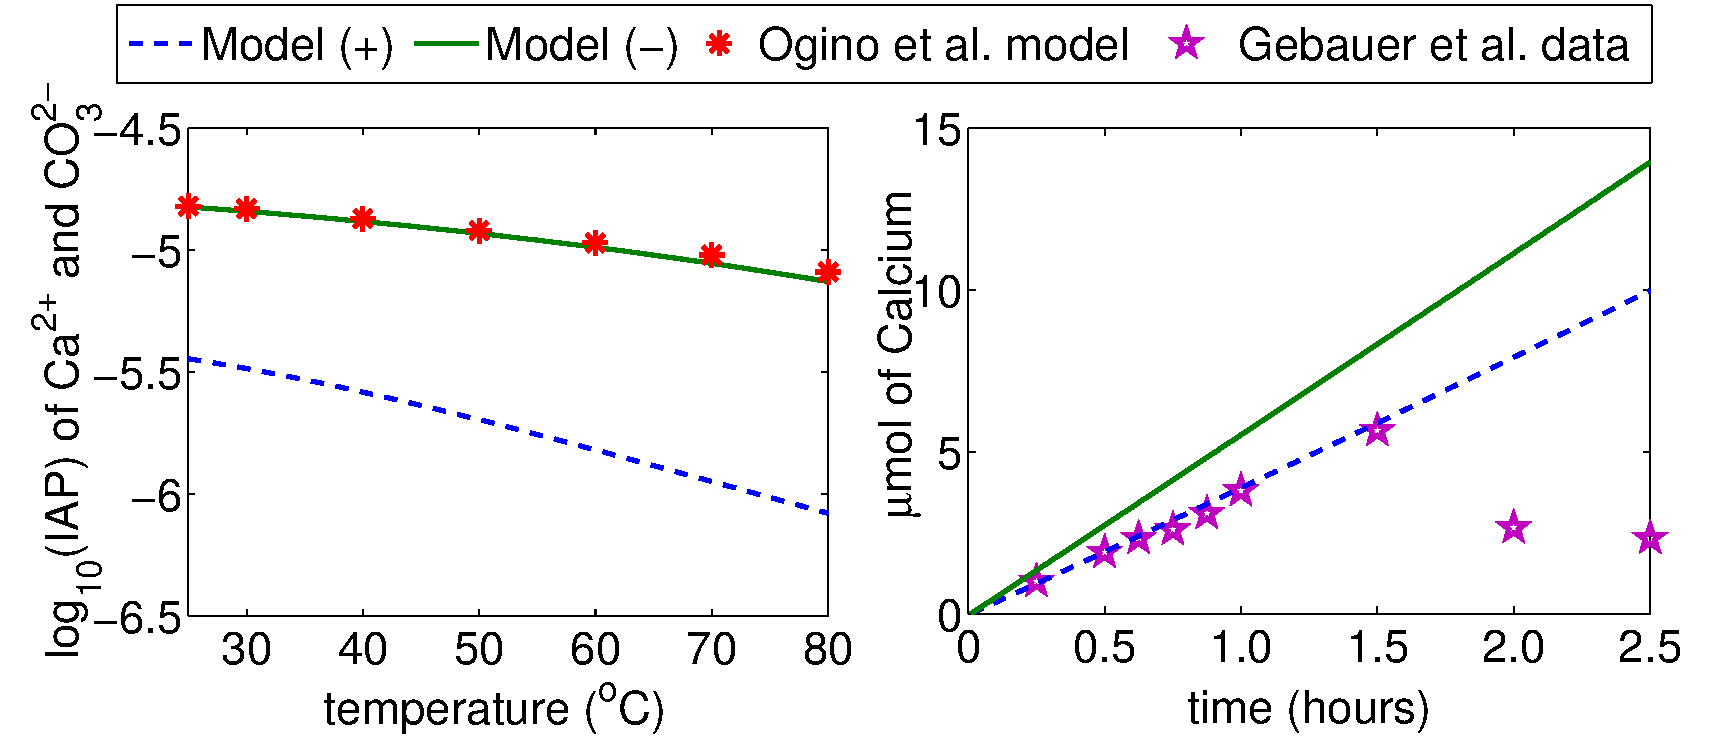
\includegraphics[scale=.5]{fig_1_Ogino_correction.pdf} 
\caption{Comparison of full \ce{CaCO3} aqueous ionic-chemistry model developed by \citet{Plummer1982} with (dashed lines - Model (+)) and without  (solid line - Model (-)) a sign error within the \ce{CaCO3}$^\circ$ equilibrium expression.  The left plot compares \citet{Ogino1987}'s IAP data (asterisks) with both models over a temperature range of 25 to $80^\circ$C, demonstrating that Model (-) was likely implemented.  The right plot compares calcium concentrations measured by \citet{Gebauer2008} (stars) with the two models over time and demonstrates how Model (+) agrees with recent experimental results.}
\label{aq_chem}
\end{center}
\end{figure}

The hypothesis that the data reported by \citeauthor{Ogino1987} needs correcting is strengthened by the right plot in Fig.~\ref{aq_chem}, which shows better agreement between the standard chemistry model with experimental data from \citet{Gebauer2008} prior to the precipitation event than the model with the imposed sign error.
%If the data published by \citeauthor{Ogino1987} is indeed inaccurate, comparison with the experimental observations becomes more challenging.
While this error effects the IAP values, it has no implications on time-scales and particle population statistics.  A simple correction can be applied when processing the experimental data.
%Thus, if this error can be accounted for, the data set can still be utilized. 
%To estimate the correct IAP of calcium and carbonate ions the two chemistry models were used to create a parametric table in terms of the extent of precipitation.  
Correlations through the extent of reaction relating \citeauthor{Ogino1987}'s apparent model to data produced in \cite{Cantera} can be observed in Fig.~\ref{chem_corr}. These correlations will be utilized during framework validation.  

\begin{figure}[h!tb]
\begin{center}
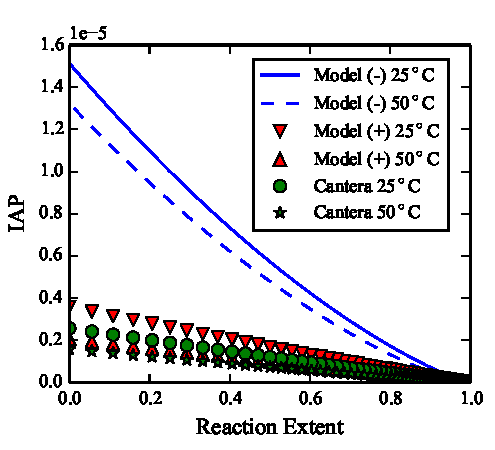
\includegraphics{fig_2_Chemistry_Correlation.pdf} 
\caption{Comparison of IAP traces over the full range of reaction extent at $25^{\circ}$C and $50^{\circ}$C calculated using an aqueous ionic equilibrium-chemistry model similar to that presented in \cite{Ogino1987} with a sign error (solid and doted lines - Model (-)), without a sign error (downward pointing and upward pointing triangles - Model (+)) and using \cite{Cantera} (dots and stars).  Chemical composition presented in \cite{Ogino1987} utilized.}
\label{chem_corr}
\end{center}
\end{figure}

%\begin{align} \label{25}
%\ln \left(IAP_{correct}^{25^\circ C} \right) =   \notag &    -0.0032450\cdot \ln(IAP_{Ogino})^3      - 0.14768\cdot  \ln(IAP_{Ogino})^2 \notag\\& %-1.3378\cdot \ln(IAP_{Ogino})   - 13.632, 
%\end{align}
%and
%\begin{align} \label{50}
%\ln \left( IAP_{correct}^{50^\circ C}\right) = \notag &   -0.0020413\cdot  \ln(IAP_{Ogino})^3 -0.096372\cdot  \ln(IAP_{Ogino})^2 \notag\\& - %%0.66910\cdot  \ln(IAP_{Ogino}) - 11.274.  
%\end{align}

%Implied meta-stable equilibrium points are implied in Ogino et al. data,  namely ACC equilibrium.  Figure \ref{fig:solubility} shows the adjusted values of \citeauthor{Ogino1987}'s equilibrium.  In general, the adjusted values are one order of magnitude lower than that reported by \citeauthor{Ogino1987}.

%The experimental initial IAP values Ogino et al. presented cannot be reproduced using their published model.   However, thy could be reproduced over a wide range of temperatures when a sign change to the fis introduced into the model.  This indicates that while \citet{Ogino1987} presented a correct model in text, in practice an error likely was committed in their BASIC equilibrium code, which overpredicts the \ce{Ca^2+} concentrations and IAP values.   \citet{Brecevic1989} and \citet{Plummer1982} measured solubility data of calcite, aragonite, vaterite, and ACC, which didn't appear consistent with the data and model presented by \citet{Ogino1987}.  By accounting for the possible error, the data presented by \citeauthor{Ogino1987} is more consistent with these referenced studies and instead shows good agreement at $25^\circ$C and improved agreement at higher temperatures.

\ce{CaCO3}  solid phases being considered, in order of increasing solubility, are: calcite, aragonite, vaterite, and ACC. The supersaturation ratio, $S_j$, of a given \ce{CaCO3} polymorph, indexed $j$, is calculated using the equilibrium solubility product, \ce{[CaCO3]_{eq}}$_{,j}$, with the activity of the aqueous-phase calcium carbonate, [\ce{CaCO3}].
%\begin{equation}\label{supersat}
%S_j=  \frac{\ce{[CaCO3]}} {\ce{[CaCO3]_{eq}}_{,j}} 
%\end{equation} 
%This description of supersaturation is equivalent to the commonly used form, where the IAP  ([\ce{Ca^2+}][\ce{CO3^2-}]) is in the numerator, because the solubility product \ce{[CaCO3]_{eq}}$_{,j}$  is corrected for this substitution.  
Temperature-dependent solubility-product correlations for the crystalline polymorphs and ACC are found in the literature \citep{Brecevic1989,Plummer1982}. 

\subsection{Time Evolution of the Particle-Size Distribution}
\label{PBE_Section}
The mathematical technique to describe the time evolution of a PSD is referred to as a population-balance equation. This method, popularized by \citet{Randolph1971}, generally allows the number distribution of particle properties (such as size) to be evolved both spatially and temporally. Commonly used within the crystallization community, population-balance equations have been shown to accurately track crystal populations for similar situations \citep{Chiang1988,Steefel1990,Hostomsky1991}.  An alternative approach recently presented by \citep{Noguera2006a,Noguera2006b} transports the time-histories of a particle population.  Such a method is valuable for precipitates whose compositions vary with time, but unnecessary for processes that lack variance of that variety and computationally more expensive than population balances for the current implementation.  Reactive transport modeling, as described by \citet{Steefel2005}, provides a holistic method of tracking mineral processes, but lacks the ability to evolve the characteristics of particle populations. 

Within our population balance, the following simplifications were made.  Based on the system setup of \citet{Ogino1987}, any spatial variations have been relegated to the mixing model (Sec.~\ref{mixing}).  Additionally, an assumption is made that greatly simplifies the description of the PSD. This assumption results from two observations: first, that aggregation has a second-order effect in this system and second, that most often the polymorph in greatest abundance has significantly more particles than any other polymorph. Based on these two observations, we neglect any cross-polymorph aggregation as a higher-order effect and can then describe the system with four separate PSDs -- one for each polymorph. In general particle systems this approximation may not hold. For the case studied here, these two observations are justified, see the results in Sec.~\ref{Results_Section}. There is another way to consider this assumption -- that even if cross-polymorph aggregation were to occur, the particles are still accounted for in the mathematical description as individuals and most of the error should then be attributed to the growth rate model.

With this assumption in place, the resulting equation for a PSD, $\eta$, as it evolves in time, $t$, is
\begin{equation}\label{generalpopulationbalance}
\frac{\partial \eta}{\partial t} + \frac{\partial}{\partial r}[G(r)\eta] =  B_{\text{N}}(r) + A(r),
\end{equation}  
where $G$ is the growth rate (also representing dissolution if it is negative), $r$ is the internal coordinate representing the radial size of the particles, $B_N$ the birth rate due to nucleation (also representing dissolution death if it is negative), and $A$ is comprised of the birth and death rates due to aggregation.

Rather than a description of the entire distribution of particle sizes, we have selected to utilize the method of moments. In precipitating systems with a small variance and a mean particle size that changes by orders of magnitude, simple sectional methods become inefficient. This inefficiency is due to the small discretization step sizes required to resolve the narrow PSD and the large number of discretization points required to span the size space. For moment methods, only a desired set of lower-order moments are solved, greatly reducing the number of calculations required. Moments contain the information necessary to calculate the mean and variance of the PSD as well as many other distribution properties. This method is accomplished by starting with the population-balance equation and transforming it into moment form, i.e. multiplying Eq.~(\ref{generalpopulationbalance}) by $r^\alpha$ and integrating over $r$, where the $\alpha^{\text{th}}$ radial moment of $\eta$ is defined as $m_{\alpha} \equiv \int_0^\infty r^\alpha \eta \, \mathrm{d}r$.  At this point the equation for the time history of the moments can be written as
\begin{equation}\label{PBE_prior_to_closure}
\frac{\partial m_\alpha}{\partial t}  - \alpha \int_{r_{\text{c}}}^\infty r^{\alpha - 1} G(r) \eta\, \mathrm{d}r =  \int_{r_{\text{c}}}^\infty r^\alpha B_{\text{N}}(r) \, \mathrm{d}r + \int_{r_{\text{c}}}^\infty r^\alpha A(r) \, \mathrm{d}r,
\end{equation}
where $r_{\text{c}}$ is defined to be the smallest radius at which particles are considered part of the system. Equation~(\ref{PBE_prior_to_closure}) generally requires a closure method due the integration of the growth and aggregation terms, which depend on an unknown distribution, $\eta$.  The quadrature method of moments (QMOM), introduced by \citet{McGraw1997}, allows for closure of these integrals. This is done by approximating the integral by Gaussian-quadrature with its associated weights, $w_k$, and abscissae, $R_k$, for each quadrature node $k = 1, 2, \dots, N$. These weights and abscissae are defined such that they satisfy the  lower-order moments:
\begin{equation}
m_\alpha = \sum_{k=1}^N w_k R_k^\alpha, \quad \text{for} \; \alpha = 0,1, \dots , 2N - 1 .
\end{equation} 
Originally derived by \citet{Gordon1968}, the product-difference algorithm can be used to solve for the weights and abscissae given the moments.  With the quadrature approximation for the growth-rate integral, the QMOM form of the equation is
\begin{equation}\label{QMOMfinal}
\frac{\mathrm{d} m_\alpha}{\mathrm{d} t}  - \alpha  \sum_{k=1}^N w_k R_k^{\alpha-1} G(R_k) =  B_{\text{N},\alpha} + A_{\alpha},
\end{equation}
where the nucleation-rate integral, $B_{\text{N},\alpha} \equiv \int_{r_{\text{c}}}^\infty r^\alpha B(r) \, \mathrm{d}r$, and the aggregation-rate integral, $A_{\alpha} \equiv \int_{r_{\text{c}}}^\infty r^\alpha A(r) \, \mathrm{d}r$, are solved according to the discussion in Sec.~\ref{Nuc_Section} and \ref{Agg_Section}.  Eq.~\ref{QMOMfinal} can be evolved through time. For initial conditions, a uniform distribution of $10^4$ particles near the size of fresh nucleates is assumed. This initial distribution is necessary for stability of the calculation, but it was ensured that this minimal number of initial particles did not effect the PSD evolution beyond a timescale of $\sim 10^{-5}$ seconds.

\subsubsection{Nucleation} 
\label{Nuc_Section}
Implementation of the classical nucleation-rate, J, takes the following form:
\begin{equation}\label{nucleationrate}
J =  z k_f C(1) C_{\text{e}}(i_\text{c}),
\end{equation} 
where $z$ is the Zeldovich factor, $k_f$ is a rate coefficient for molecular growth of a cluster, $C(1)$ is the number density of single precipitant molecules in solution, and $C_{\text{e}}(i_\text{c})$ is the equilibrium-based number density of clusters at the critical size \citep{Kashchiev2000}. The embryonic-cluster size distribution is modeled as a Boltzmann distribution.  When solving for the embryonic-cluster size distribution, the Gibbs free energy of the cluster, $G$, must be first solved, which is set relative to a single molecule in order to maintain self consistency \citep{Girshick1990,Kashchiev2000}.  
\begin{equation}
\Delta G(i) = -k_\text{B} T \ln (S)(i-1) + (36 \pi \nu^2)^{1/3}\sigma(i^{2/3} - 1)
\end{equation}
This change in Gibbs free energy describes the energy loss due to increased volume of the new phase versus energy gain from the enlarged surface area of the interface between phases. The Zeldovich factor, originally derived by \citet{Zeldovich1942}, helps correct for the fact that the Boltzmann distribution assumes equilibrium, yet nucleation occurs due to deviations from equilibrium.  \citet{Katz1977} provides an alternative viewpoint on the embryonic cluster distribution.

There are a variety of expressions for the forward reaction-rate coefficient, but two forms commonly used and that were explored throughout the framework development are the interface-transfer-limited and diffusion-limited models  found in \cite{Kashchiev2003}. %The diffusion-limited version is utilized to maintain consistency with the growth models. 

Subtleties in the definition of the nucleation-rate can have significant implications on the population-balance equation, the nucleation-rate expression itself, and the coupling with the aqueous-phase equilibrium chemistry. With this in mind, we carefully word the definition of nucleation-rate as the quasi-steady flux of embryonic clusters as they grow into particles that are then tracked by the PSD. For this hand-off of pre-nucleate clusters to nucleated particles, we have followed the established convention of using the thermodynamic critical cluster size, $i_{\text{c}}$, which occurs when $\frac{\mathrm{d} \Delta G(i)}{\mathrm{d}i} = 0$.  Due to the use of size-dependent interfacial tension, as will be elaborated upon in Sec.~\ref{interfacial_tension}, a quadratic version of the Kelvin equation \citep{Dirksen1991} must be solved.
%Here stability is defined with regards to single molecule addition. This critical size is determined from the Kelvin equation \citep{Dirksen1991} as
%\begin{equation}\label{Kelvin}
%i_{\text{c}} = \frac{32 \pi \nu^2 \sigma^3}{3 ( k_\text{B} T \ln S )^3} ,
%\end{equation} 
%where $\nu$ is the molecular volume, $\sigma$ is the interfacial tension, $k_{\text{B}}$ is the Boltzmann constant, and $T$ is the temperature. 
The critical size, written as the number of molecules in a cluster, must correspond to the PSD domain boundary, $r_\text{c}$.  We relate the two through an assumed spherical shape ($i_{\text{c}}=\frac{4 \pi}{3 \nu}r_{\text{c}}^3$).  Also, when a particle nucleates and begins to be accounted for within the PSD, the molecules comprising that particle can no longer contribute to the molecular concentration in solution and the equilibrium chemistry is updated to conserve mass.

A secondary heterogeneous-nucleation mechanism \citep{Kashchiev2003} was also explored. Secondary heterogeneous nucleation allows for nucleation on particles already present in the system and introduces additional unknown model parameters such as: the contact angle at which one polymorph nucleates on particles of each of the other polymorphic forms, and the density of nucleation sites for each polymorphic form.  A discussion of the implications of heterogeneous nucleation is included in Sec.~\ref{Model_Alternatives}.

The quasi-steady nucleation model assumes that the distribution of pre-nucleation clusters is fully established. This is certainly not true for infinitely fast mixing and may not be accurate for finite mixing rates. When the \ce{Ca^2+} and \ce{CO3^2-} containing solutions are mixed, individual \ce{CaCO3} molecules are formed and the distribution of embryonic clusters evolves toward its quasi-steady state. For timescales near the mixing rate, the embryo distribution will be more heavily weighted to smaller sized clusters. The period of time before reaching the quasi-steady nucleation-rate is referred to as the time lag or induction time. Transient nucleation models describing nucleation during the ramp-up process,  examples of which can be found in \cite{Kelton2010}, have been investigated.  The most well known model is that by \citet{Kashchiev1969},
\begin{equation}
J(t) = J \bigg[1+ 2 \sum_{m=1}^\infty (-1)^m exp(-m^2 \frac{t}{\tau})\bigg],
\end{equation}
where $\tau = 4/z^2 \pi^3 k_f N(1)$ is the induction time \citep{Kelton1983}.  The nucleation ramp up was only investigated for infinitely fast mixing. There is currently no theoretical model for simultaneous finite mixing rate and nucleation time lag.

With the physical theory of nucleation in place, it must be incorporated into the population-balance equation. The physical description above implies a boundary condition flux, but this is mathematically equivalent to a  delta-function source term at the boundary.  The birth-rate due to nucleation is then related to the nucleation-rate itself by
\begin{equation}
B_{\text{N}} = \delta(r-r_{\text{c}}) J .
\end{equation}
The nucleation-rate integral is given as
\begin{equation}
B_{\text{N},\alpha} \equiv \int_{r_{\text{c}}}^\infty r^\alpha B_{\text{N}}(r) \, \mathrm{d}r = r_{\text{c}}^\alpha J .
\end{equation}

Based on the recent progress regarding the possibility of non-classical nucleation for ACC \citep{Gebauer2008,Rodriguez-Blanco2011}, an ideal mathematical description would incorporate a non-classical nucleation mechanism for ACC and classical nucleation for vaterite, aragonite and calcite. Currently, there is no well-established mathematical description for the non-classical nucleation-rate. Consequently and in accordance with the scope of the current investigation, classical nucleation has been selected as a surrogate for the non-classical nucleation-rate.

\subsubsection{Growth}
\label{Grow_Section}
Particle growth can follow many possible mechanisms depending upon environmental and particle-material properties. Common mechanisms include monosurface nucleation, polysurface nucleation, screw dislocation, among others.  For a comprehensive review see \citet{Dirksen1991} and \citet{Lasaga1998}.  While many mineral growth rates are presented as surface area normalized, such rates can be converted into a radial basis through mathematical manipulation.  Due to large changes in the system's supersaturation, different growth mechanisms may be exhibited for each of the polymorphs as their respective bulk supersaturations transition from high to low.  A brief review of the mechanisms considered for the current application follows.

Initially the system is highly supersaturated with respect to all polymorphs.  At this point the surface growth rate is fast with an unknown kinetic rate expression, but the overall rate is limited by diffusion of precipitant molecules to the surface of the particle \citep{Kawano2002}. This mechanism is known as diffusion-limited growth, assumes equilibrium boundary conditions, and can be described mathematically as
\begin{equation} \label{diffgrowth}
G(r) = \frac{D }{\rho r} \ce{[CaCO3]_{eq}} (S-\bar{S}),
\end{equation}
where $D$ is the diffusion coefficient, $\rho$ is the polymorph's molar density, and $\bar{S}$ is a ratio of activities \citep{Nielsen1964}.  The ratio $\bar{S}$ is the activity of a finite-radius particle normalized by the activity of an infinite-flat surface.  Although $\bar{S}$ is often assumed as unity, it can be derived from the Kelvin equation \citep{Dirksen1991,Noguera2006a} and results in Ostwald ripening effects upon small particles:
\begin{equation}
\bar{S} \equiv e^{2 \sigma / \rho R T r} .
\end{equation}
The diffusion coefficient is  assumed to be linearly dependent on temperature [$ 2.4533\times 10^{-11}(T - 273.15 ) + 4.9467\times 10^{-11} [\text{m}^2 \text{s}^{-1}$]]\citep{OLI}.  The expression for diffusion limited growth, Eq.~(\ref{diffgrowth}), assumes a spherical particle geometry. While this  is a good approximation for most of the polymorphs, aragonite is known to form crystals with greater resemblance to cylindrical geometries.  A similar diffusion-limited growth model for cylindrical particles was used,
\begin{equation} \label{cyl_diffgrowth}
G(r) = \frac{7}{6\ln(2)}\frac{D }{\rho r } \ce{[CaCO3]_{eq}}(S-\bar{S}).
\end{equation}
Within the cylindrical diffusion-limited growth model, it was assumed that the diameter-to-height aspect ratio of the crystals is roughly one to six and that the concentration boundary layer of the particles is on the order of the particle size.

Once the supersaturation ratio reduces to levels closer to $\bar{S}$, it has been shown that \ce{CaCO3} polymorphs grow by a surface controlled rate, such as the screw-dislocation mechanism, for the pH range of interest \citep{Kralj1997,Collier1999,Andreassen2004,Andreassen2005,Andreassen2010,Noiriel2012}. Singular screw dislocation can be  described mathematically as
\begin{equation}\label{surface_growth}
G(r) = K_r (S-\bar{S})^2 \quad \text{when} \quad S > \bar{S} ,
\end{equation}
where $K_r$ is an empirical reaction-rate constant \citep{Kralj1990}, while the multi-source equivalent has a linear dependence on chemical affinity \citep{Noiriel2012}. Each polymorph has a unique rate constant whose temperature dependence is incorporated using the Arrhenius equation due to being reaction limited \citep{Lasaga1998}.  Screw dislocation growth constants for vaterite and calcite were documented by \cite{Kralj1990,Kralj1997} and by \cite{Romanek2011} for aragonite.  While affinity based models for surface controlled rates are widely used, many reaction rate based models also capture the phenomena well \citep{Plummer1978,Shiraki1995}.

Although there is has been a great deal of research investigating surface defect controlled growth mechanisms of the crystalline polymorphs such as \citet{Kralj1990,Kralj1997,Gutjahr1996}, it has also been found that the controlling growth mechanism switches to 2-D surface nucleation  as the supersaturation increases \citep{Teng2000,Noiriel2012}.  As described by \citet{Dirksen1991}, while the supersaturation rises, the controlling growth mechanism will continue to change until diffusion limited growth is reached.  Although all appropriate growth mechanisms could be implemented within the framework, with the uncertainty in the selection of a growth mechanism -- further complicated by the possibility of switching from  one mechanism to another -- diffusion limited growth was primarily applied to all three crystalline polymorphs. The implications of this selection are given  in Sec.~\ref{Model_Alternatives}.  There is currently little known about how ACC grows at similar supersaturation levels. Diffusion limited growth is judged to be a viable mechanism for ACC due to the lack of crystal structure and high rates of growth.  
%,  such as polysurface nucleation or screw dislocation, involve limiting steps during the incorporation of new  molecules into the crystal structure, but how or if these mechanisms would be applicable to ACC is unclear.  

Recently, there has been a great deal of new research published on calcite growth mechanics.  Papers by \citet{Stack2010,Gebrehiwet2012,Bracco2013} have found calcite's growth rate to be largely effected by not only the supersaturation, but also by the ratio of the ions.  The effect of the solution's pH upon the limiting growth mechanism has also resurfaced as an area of intrigue \citep{Ruiz-Agudo2011}.  \citet{Wolthers2012} explored these issues simultaneously and their model was explored within the framework at supersaturation values near $\bar{S}$. 

\subsubsection{Dissolution}
\label{Dissolution_Section}
As the precipitation process advances in time it displays two phenomena: Ostwald-ripening \citep{Lifshitz1961} and Ostwald's step rule \citep{Ostwald1897} as it applies to polymorphs. In terms of the mathematical description of  Eq.~(\ref{generalpopulationbalance}), dissolution appears twice. First, dissolution appears as a negative growth term, $G(r) < 0$. And second, when a particle shrinks beyond the smallest size considered in the PSD, dissolution appears as a death term. This death is equivalent to a negative nucleation event, $B_{\text{N}} < 0$.

Dissolution in the form of negative growth occurs for undersaturated solutions ($S < 1$), but it may also occur for supersaturation ratios larger than unity if the particle is small enough that the size-effect of the Kelvin equation results in unfavorable energetics.  Dissolution rates within \ce{CaCO3} system have been found to be limited by the growth rate of more stable polymorphic forms \citep{Ogino1990,Kralj1997,Rodriguez-Blanco2011}.  That being said, our approach for vaterite and aragonite's dissolution rates, is to use the diffusion limited mechanism, which is the same as Eq.~\ref{diffgrowth}/\ref{cyl_diffgrowth}, in order to allow aragonite and calcite's growth rates dictate the system dynamics.  
%Diffusion limited dissolution rates are sufficiently fast to insure the system does not become limited by the dissolution of metastable forms.  
Although \cite{Kralj1994} reported vaterite's dissolution to be diffusion limited, \cite{Chou1989} found aragonite's dissolution to be limited by surface kinetics.  Due to the lack of temperature dependent model parameters presented by \citet{Chou1989}, diffusion limited dissolution is the best option available for aragonite.  Calcite's dissolution mechanism has been established as being surface reaction limited for the validation data's pH range \citep{Chou1989,Gutjahr1996,Cubillas2005} and temperature dependent parameters are available \citep{Plummer1978}.  

%That being said, our approach is to represent dissolution using the more certain growth mechanisms but with a negative driving force %to mimic particle shrinking.  For diffusion-limited growth, Eq.~(\ref{diffgrowth}), the condition of $S < \bar{S}$ automatically results in a %negative  growth rate \citep{Kralj1997}. This behavior is not true for the screw-dislocation mechanism, and a negative sign must be %added explicitly:
%\begin{equation}
%G(r) = -K_r (S-\bar{S})^2 \quad \text{when} \quad S \leq \bar{S} .
%\end{equation}
%\citep{Cubillas2005}

ACC's dissolution mechanics are still an area being explored.  Some literature suggests that ACC directly crystallizes into other forms or occurs in combination with dissolution \citep{Rodriguez-Blanco2011,Bots2012}.  Due to the current ambiguity, diffusion limited and surface limited dissolution mechanisms with fitted rate constants were explored.
%Again, a variety of combination of mechanisms were attempted and the implications are described in Sec.~\ref{Results_Section}.

Dissolution in the form of a negative birth term allows for particles to be removed from the PSD.  Historically this death term has presented challenges for QMOM methods, and recent progress in this regard has been made by \citet{Yuan2012}. The negative growth type of dissolution has a primary effect on the system under consideration and the dissolution-death term has a negligible effect.  We have taken a pragmatic approach of selecting the left boundary of the PSD and specifying a death rate.  The selection of the PSD's left boundary must be a value small enough that the specified dissolution-death rate shows negligible impact on the equilibrium chemistry.  Within the current framework implementation, a particle radial size of $6 \times 10^{-2} \mu m$ and a respective distribution weight of $10^{-2} \; \# / m^{3}$ were chosen to specify the left boundary.

\subsubsection{Aggregation}
\label{Agg_Section}

Aggregation does not have a primary influence on the variables reported by \citet{Ogino1987} -- explicitly on the system characteristics IAP and polymorphic abundance. These two quantities provide a good measure of the physical state of \ce{CaCO3}, if it is in the aqueous-phase or precipitated as one of the polymorphs, but do not characterize the size of the particles. However, in the dynamic evolution of the system, aggregation can have an indirect effect on these variables through the size dependence of growth and dissolution. Irrespective of these variables, the degree of aggregation in the system of interest is minor. Nonetheless, aggregation has been included in this study for two reasons: for completeness in the theoretical description and for the flexibility of this framework in it applicability to similar systems.

We adopt a QMOM form of the aggregation term as derived by \citet{Marchisio2003}:
\begin{equation}\label{aggreagtioneq}
A_{\alpha}  \approx \frac{1}{2} \sum_{i=1}^N w_i \sum_{j=1}^N \beta(R_i,R_j)  w_j (R_i^3 + R_j^3)^{\frac{\alpha}{3}} - \sum_{i=1}^N R_i^{\alpha} w_i \sum_{j=1}^N \beta(R_i,R_j) w_j ,
\end{equation}
where $\beta$ represents the aggregation kernel. This aggregation kernel is the product of a collision frequency, $\beta^*$, and a collision efficiency, $\Psi$, \cite{Liew2003}.
\begin{equation}
\beta (r_i , r_j ) = \beta^*  (r_i , r_j) \Psi ,
\end{equation}
A Brownian motion frequency kernel, found in \citep{Elimelech1995}, was implemented to capture the aggregation of the large quantity of small particles created within the validation system.
%We have selected to include collisions due to both Brownian motion and isotropic turbulent shear. These two collision %mechanisms are approximated as being additive for the present implementation.
%\begin{equation}
%\beta^* (r_i , r_j) = \beta_{\text{Brownian}}^* + \beta_{\text{Turbulent Shear}}^*
%\end{equation}
%Models for these collision frequency kernels are found in \citet{Elimelech1995} and \citet{Marchisio2003}, respectively. 
While collision frequencies are fairly well defined within the literature, the collision efficiency is an area of research still being explored.

Collision efficiency, $\Psi$, must be considered because not all collisions result in aggregation. Fundamentally, the collision efficiency can be thought of as the probability that the bonding forces overcome tensile and shear stresses.  Numerically it can range from one, where all collisions result in aggregation, to zero. 
%At low ionic strengths the balance between attractive and repulsive forces influences the efficiency, but at high ionic strengths the repulsion greatly diminishes and the efficiency approaches unity \citep{Marchisio2003}.
 A semi-empirical method introduced by \citet{Hounslow2001,Liew2003,Andreassen2004} based upon particle growth rates and physics strength properties, which has been explored in recent literature \citep{David2003,Ilievski2006}, is used for the current application.

\subsubsection{Interfacial Tension}
\label{interfacial_tension}
Interfacial tension plays a crucial role in the dynamics of the system.  The value of interfacial tension has an predominate influence on the nucleation-rate, is a minor factor in the growth and dissolution rates (through the Kelvin equation -- affecting Ostwald ripening), and can influence the aggregation-rate. 
There is wide variability for reported values of interfacial tension from the literature \citep{Goujon1976,Sohnel1982,Christoffersen1990,Nancollas1999,Donnet2009}. 
%Some values are reviewed in Table~\ref{tension_table}. 
The variety of reported values is likely a result of differing measurement techniques and experimental methods.  These values are either reported for one set of conditions or averaged, while the framework aims for validity over significant changes in composition and temperatures.
%\begin{table}[ht]
%\caption{A review of values for interfacial tension adapted from \cite{Donnet2009}}
%\centering
%\begin{tabular}{c | c | c | p{8cm} c }
%\hline\hline
%Polymorph & $\sigma [\text{mJ} \; \text{m}^{-2}]$ & Temp. [$^\circ$C] & Source \\ 
%\hline
%ACC & -- & -- & Not well established\\
%Vaterite & $6.8 - 133$ & $10 ^\circ - 45 ^\circ$C & \citep{Sohnel1982,Manoli2000,Kralj1990,Morales1996,Donnet2009} \\
%Aragonite & $150$ & $25 ^\circ$C  & \citep{Sohnel1982} \\
%Calcite & $19.5 - 280$ & $20 ^\circ - 25^\circ$C  & \citep{Christoffersen1990,Sohnel1982,Goujon1976,Holysz1994,Morales1996} \\
%\hline
%\end{tabular}
%\label{tension_table}
%\end{table}

With a need for correct values of interfacial tension, accurate to within $<1\%$ due to nucleation's sensitivity, we have turned to thermodynamic theory. Characterization of interfacial tension in an ionic solution that is varying in temperature and composition is known to be a complex problem. The Gibbs' absorption equation, Eq.~(\ref{gibbsadsorption}), demonstrates dependencies on the specific excess entropy, $S_a^E$, and the chemical potential, $\mu_i$. Ionic solutions further complicate this description due to the need to understand the molecular interactions occurring between the ions in solution and the particles in order to describe the excess surface concentration, $\Gamma_i$.
\begin{equation} \label{gibbsadsorption}
\mathrm{d} \sigma = -S_a^E \mathrm{d} T - \sum_i \Gamma_i \mathrm{d} \mu_i 
\end{equation}

Following an approach similar to that of \citet{Mersmann1990}, but maintaining the temperature dependent term, interfacial tension can be expressed as
\begin{equation}\label{FullInterfacialTensionEq}
\sigma(T,\mu) = \sigma(T_\circ,\mu^\circ) - S_a(T-T_\circ) - 0.414k_BT(\rho N_A)^{2/3} \ln \bigg(\frac{S[\ce{CaCO3}]_{eq}}{K}\bigg),
\end{equation}
where $T_\circ$ and $\mu^\circ$ are the reference temperature and chemical potential respectively and $K$ is aqueous equilibrium constant for \ce{CaCO3} and its comprising ions.  The term $0.414k_BT(\rho N_A)^{2/3}$, is an approximation of the the excess surface concentration, as derived by \citet{Mersmann1990}.  A more precise characterization of the surface concentration with adsorption models could be implemented, such as was done by \citet{Donnet2009}, but is currently neglected.  Utilizing this model allows for two parameters, $S_a$ and $\sigma(T_\circ,\mu^\circ)$, to be fit for each \ce{CaCO3} form and provides a model with both temperature and composition dependence.  Other models with similar capabilities exist, such as that of \citet{VanOss_2006}, but \citeauthor{VanOss_2006}'s model requires more fitting parameters.  

%For our application, we assume that the concentration dependent term can be dropped, and this results in an equation that is linear in temperature. We have elected to fit the linear parameters to the data. Models such as those presented in \citet{Mersmann1990} and \citet{VanOss_2006} provide both temperature and composition dependence, however they require many more fitting parameters.

Although the idea that particle properties deviate from bulk-phase properties on the nano-scale has long been discussed, it has recently gained traction with the surge in nano-scale research. Size-dependent interfacial tension was originally modeled by \citet{Tolman1948} as 
\begin{equation}\label{tolmanEquation}
\sigma = \sigma_\infty \bigg( 1 - \frac{2 \delta_T}{r}\bigg) ,
\end{equation} 
where $\sigma_\infty$ is the bulk phase interfacial tension and $\delta_T$ is the Tolman length. A Tolman length of $0.2 \times r_1$ as recommended by \citet{Kalikmanov1997}, where $r_1$ is the molecular radius, is utilized in the current implementation. The Tolman length presents another contribution to uncertainty in the results. Determination of this value is still an active area of research.  Size-dependent interfacial tension causes the preliminary critical cluster size of particles required for nucleation to decrease or larger fitted interfacial tension parameters. This effect creates a greater initial burst of nucleation activity.

\subsection{Coupling Equilibrium Chemistry and Particle-Size Distribution} 
\label{Spec_Bal_Section}
Changes in the PSD need to be reflected in the composition of the aqueous-phase, which in turn is coupled back to the evolution of the PSD.  In order to accomplish solid-liquid coupling, changes in both the solid and liquid phases are related to a reaction-extent variable, $\chi$.  This reaction extent is defined as a normalized amount of precipitated \ce{CaCO3} irrespective of polymorphic form.  The material amount represented by each polymorph individually is simply the polymorph's molar density, $c_j$, multiplied by the polymorph's total volume, $v_j$.
\begin{equation}
c_j v_j = \frac{4 \pi c_j}{3} \int_{r_1}^{\infty} r^3 \eta_j \, \mathrm{d}r = \frac{4 \pi
  c_j}{3}m_{3,j}
\end{equation}
This equation assumes a spherical shape, so special care must be taken for translating this into a cylindrical interpretation for aragonite. The total amount of material in the solid phase is calculated by summing over all the polymorphs, and the extent of reaction is calculated by normalizing the total amount by its maximum.
\begin{equation}
\chi = \frac{4 \pi }{3}\sum_j\frac{c_j m_{3,j}}{n_{\text{$\ce{CaCO3}$},\text{max}}}
\end{equation}
The maximum, $n_{\text{$\ce{CaCO3}$},\text{max}}$, is easily determined from the stoichiometrically limiting ion.  Thus, the rate of change of the reaction extent is proportional to the sum of  rates for the third moments, which are already calculated in the QMOM.
\begin{equation}
\frac{ \mathrm{d}\chi}{\mathrm{d}t} \propto \sum_j c_j \frac{\mathrm{d} m_{3,j}}{\mathrm{d} t} 
\end{equation}

With a value for the extent of reaction, the available amount of \ce{Ca^2+} and \ce{CO3^2-} become constraints in the calculation of the aqueous-phase equilibrium. The equilibrium calculation then provides the necessary value of supersaturation for each of the polymorphs, effectively completing the phase coupling.  Parameterizing the aqueous-phase equilibrium evolution by a single variable allows the equilibrium calculations to be performed separately with results tabulated according to reaction extent.

\subsection{Mixing}
\label{mixing}
Imperfect mixing is often neglected when analyzing precipitation processes. This approximation seems unfounded since even fast mixing timescales ($10^{-3}-10^{-1}$ seconds) will be significantly slower than the nucleation timescales ($10^{-7}-10^{-4}$ seconds) for \ce{CaCO3} with high supersaturation ratios.  Thus mixing will be the rate limiting process. The experimental system was described as one liter vessels being mixed with magnetic stirrers and no difference was noted when a screw propeller-spindle was used \citep{Ogino1987}.  A mixing model can be utilized to capture the effects on the system's composition profiles during the mixing period.  A more detailed description of mixing would require additional information about the experimental setup and conditions. For the simulations performed here, a three-environment model~\citep{Fox2003} was selected with a specified mixing time.  The three-environment mixing model initiates with two mixing environments, which represent the two feed streams of the experiment, and then redistributes these two streams into the third mixing environment over time. This mixing model is known to be simplistic because it does not explore the full spectrum of possible compositions, but it does capture the most important implications of mixing.  A conservative range of mixing timescales for the one-liter vessel with a magnetic stir bar was explored, from $10^{-1}$ to $10^2$ seconds. Implications of the selection of mixing timescale are discussed in Sec.~ \ref{Results_Section}.  There is currently no theoretical model for simultaneous finite mixing rate and nucleation time lag.

\section{Results}
\label{Results_Section}
To validate and test the predictive capabilities of the framework described in Sec.~\ref{theory}, we compared our results with those obtained from experiments conducted by \citet{Ogino1987}.  Utilizing the temperature and initial system chemical composition description provided by \citeauthor{Ogino1987}, system evolutions were calculated.  Experimental data was presented primarily in two forms: the temporal evolution of volumetric polymorphic abundances and IAP traces.  Our framework can output data in these same forms by calculating the IAP within the equilibrium-chemistry calculations and using the evolution of the third moments to track polymorph total volumes.  Interfacial tension values were the major source of uncertainty.  The framework presented can generate many outputs, not all of which has corresponding validation data, that are of interest within precipitation studies.  Such output variables will be discussed first.  Next, examples of framework configurations will be discussed and compared to experimental data.   Variation is compared to a canonical configuration.  Finally, the chosen system configuration had parameters for the interfacial tension equation, Eq.~\ref{FullInterfacialTensionEq}, optimized and the results are analyzed.  General system variables not specified previously are tabulated below.

\begin{table}[ht]
\caption{Properties used within framework}
\centering
\begin{tabular}{ p{5cm} | c | p{2cm}  }
\hline\hline
Polymorph Density$^1$* & $[1.9, 2.64, 2.94, 2.71] \times 10^6 $ & $ [\text{g} \; \text{m}^{-3}]$     \\
Fluid Density & $998.2 $ & $ [\text{kg} \; \text{m}^{-3}]$  \\
Fluid Dynamic Viscosity & $1.002\times 10^{-3} $ & $ [\text{kg} \; \text{s}^{-1} \; \text{m}^{-1}]$    \\
Mixing Time & $0.75$ & $[ \text{s} ]$  \\
Turbulent Dissipation Energy & $5000$ & $[ \text{J} \; \text{kg}  ]$  \\
ACC Dissolution Constant & $9\times 10^{-9}$ & $[\text{m} \; \text{s}^{-1}]$ \\
\hline
\end{tabular}
\text{* \textit{ACC, Vaterite, Aragonite, Calcite}} \hspace{2cm}
\text{$^1$ \cite{Faatz2005}, \, \cite{Anthony2001} }
\label{properties_table}
\end{table}

\subsection{General Results}
\label{General_Results}

Utilizing a moment method to track the solid phase evolution of the precipitation system provides many forms of useful data that are not being utilized in the current framework validation, but could be insightful for similar applications.  Evolving the moments of the particle distribution allows for means, variances, and other statistics of the particle population to be easily calculated at any time throughout the simulated temporal period, potentially allowing for other avenues of verification with experimental data.  Examples of the available distribution characteristics provided by moment methods include the evolution of the number of particles, average size, as well as size variance as is shown in Fig.~\ref{avgradius} and Fig.~\ref{std_S}.  The optimized framework configuration described in Sec.~\ref{Model_Results} was utilized to create these examples.  Simultaneous tracking of the solid-phase PSD and the aqueous-phase ionic equilibrium-chemistry allows for correlations between events in the two phases as the supersaturation traces in Fig.~\ref{std_S} will be shown to demonstrate.

\begin{figure}[h!tbp]
\begin{center}
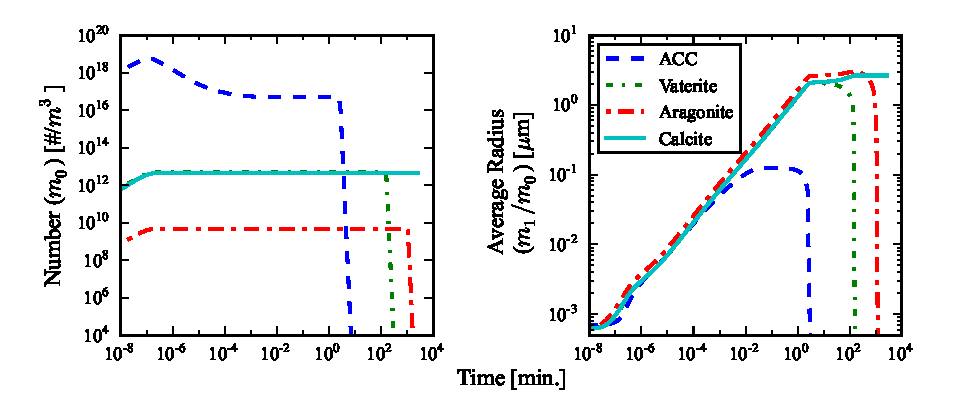
\includegraphics{fig_3_number_and_average_radius}
\end{center}
\caption{Framework calculated $0^{\text{th}}$ moment, $\textit{m}_0$, (or particle number density) traces over time on the left and average radial size, $\textit{m}_1/\textit{m}_0$, traces over time on the right for four \ce{CaCO3} polymorphs at $25^\circ$C.  ACC is shown with the dashed line, calcite with the solid line, and vaterite and aragonite with the dash-dot lines, where vaterite's dash-dots are shorter than aragonite's.  These are examples of available data from the QMOM method of calculating PSD evolutions.} 
\label{avgradius}
\end{figure} 
Both plots in Fig.~\ref{avgradius} display an initial period of nucleation and mixing for all polymorphs until around $10^{-7}$ minutes.  After nucleation, the total number traces level out while the average radii continue to increase, indicating that growth with mixing is occurring.  An exception to that trend in noted for ACC, which experiences significant aggregation.
\begin{figure}[h!tbp]
\begin{center}
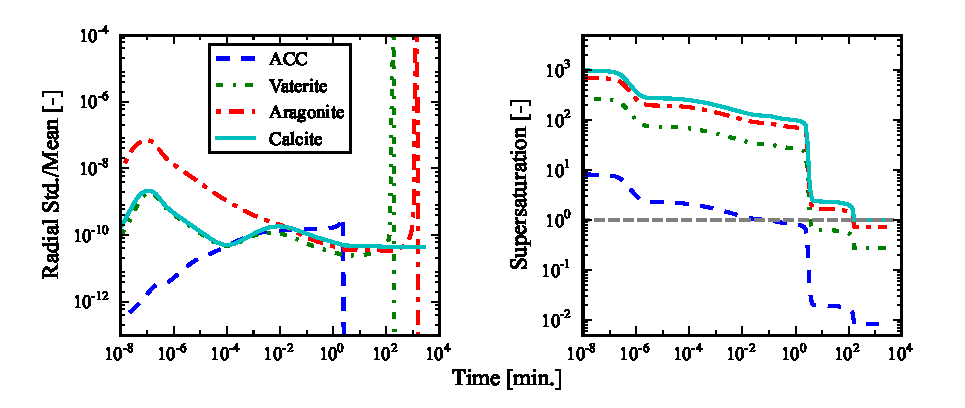
\includegraphics{fig_4_standard_deviations_and_supersaturations}
\end{center}
\caption{Framework calculated polymorph PSD standard deviation traces normalized by their respective means shown throughout time are on the left and the respective supersaturation traces over time are on the right.  ACC is shown with the dashed line, calcite with the solid line, and vaterite and aragonite with the dash-dot lines, where vaterite's dash-dots are shorter than aragonite's.  A supersaturation line at a value of 1 is shown as dashes, smaller and more frequent than ACC's, and this line is meant as a reference frame by which the driving force of physical phenomena can be judged.}
\label{std_S}
\end{figure}
Within the radial standard-deviation plot (Fig.~\ref{std_S}) there is also a distinct upward slope for all polymorphs during the mixing- and nucleation-dominated time frame.  This slope deviates to downward once growth takes over as the dominating mechanism.  The initial standard deviations become larger due to nucleation occurring at a varying critical size, which itself spans an order of magnitude.  Yet, it should be pointed out that these normalized standard-deviations are all small, indicating narrow distributions.  The slope in the standard deviation traces are continually negative throughout periods dominated by diffusion-limited growth.  This is due to diffusion-limited growth being size dependent, causing the smaller particles to grow faster than the larger particles, effectively collapsing the PSD.  In contrast, aggregation based growth increases PSD standard-deviations.  Aggregation based growth primarily effects ACC, but also vaterite and calcite to lesser extents ($\sim$5$\times$10$^{-4}$-10$^{-2}$). Comparing the supersaturation plot with the particle number density, it can be noted that growth, not nucleation, has a far greater effect upon the system's supersaturation and is the major means of phase transformation occurring within the system.

Now focusing on ACC's radial standard-deviation and supersaturation curves, its supersaturation drops during growth.  Mixing limits growth between $\sim$10$^{-5}$-10$^{0}$ seconds.  Once the supersaturation levels out near a value of one, the driving force behind the growth is no longer present.  This holds first for the smaller particles, then for the progressively larger particles.  This correlates with the slightly positively sloped region in ACC's radial standard deviation, demonstrating that growth has indeed ceased and dissolution began for the smaller particles.  Next, as the region of the PSD (where there is a driving force for dissolution) increases, Ostwald ripening results in the large spike in the radial standard deviation.   As the other polymorphic forms continue to grow throughout ACC's dissolution and coalescence, the entire ACC PSD becomes energetically favorable for dissolution, and the radial standard deviation drops off as all of the ACC particles are dissolved away.  Without the aqueous ionic equilibrium-chemistry model to couple the four PSDs, dissolution dynamics could not be captured because the growth of the other polymorphic forms is the major driving force behind ACC's rapid dissolution.  The same general PSD evolution then occurs for vaterite and aragonite, eventually leaving only calcite to experience Ostwald ripening until an equilibrium is reached.  It can be noted that aragonite's dissolution does not have a corresponding drop in the supersaturation traces due to the minimal relative abundance of it present in the system at $25^\circ$C. 

The average radial-size plot illustrates how particle removal occurs only after particles of the represented abscissa have mostly dissolved and the average radial size is dropping quickly by that point in time.  The removal of particles from the system, as mentioned in Sec.~\ref{Dissolution_Section}, can be noted in the plot of the particle number density. The linear downward slope is present because the non-physical death kernel implemented was specifically designed to have a linear slope in log-log space.  Again, care has been taken that particles are sufficiently small that the shape of this death kernel has negligible effect ion the equilibrium chemistry or the remaining polymorphs.   

Although particle size characteristics were not tabulated by \citeauthor{Ogino1987}, figures containing scanning electron micrographs photos were included.  \citeauthor{Ogino1987}'s Fig. 5-h depicts vaterite and calcite particles at 50 minutes under 25$^\circ$C conditions.  The vaterite and calcite particles shown had radii around two microns, which the calculated averages are in reasonable agreement.  At these same conditions  \citeauthor{Ogino1987}'s Fig. 5-e shows ACC's particles, seven minutes into the experiment, to range from around .5 to 2 $\mu m$.  Although this range does not overlap with the calculated average radii value of $\sim$0.1 $\mu m$, being within an order of magnitude was satisfactory when there is such uncertainty in the nucleation and growth mechanism. 

\subsection{Alternative Configurations}
\label{Model_Alternatives}
While the aim of the current approach is to implement a basic framework that is able to capture the system's dynamic trends, many possible alternative configurations were mentioned within Sec.~\ref{theory}, Theory, and these alternatives were explored throughout the framework development.  When choosing the number of quadrature nodes, initial simulations were run with two and three nodes.  Although the results produced were similar,  there were significant enough differences to justify exploring the use of more nodes.  With four or five nodes, no differences were noted compared to the case of three nodes.  This corresponds to evolving up to ten moments of each PSD.  Thus three quadrature nodes were used in the final framework for computational speed.  

Within the nucleation model a diffusion-limited reaction-rate coefficient was ultimately chosen for the final framework, but an interface-limited variation was also explored.  The interface-limited reaction-rate coefficient produced results similar to the diffusion-limited variation and the fitted interfacial-tension reference points and the excess entropy values were within 0.01$\%$ and 2.0$\%$ respectively of the optimized diffusion-limited values.  Similar behavior was observed by \citet{Lindenberg2009}.

The time before the two solutions were considered fully mixed was also explored.  During the optimization process of the final framework, a range of mixing times were surveyed and a mixing time that allowed for the majority of the mixing to occur prior to $1.5$ second, with complete mixing around $5.0$ seconds was selected.  This mixing time allowed for the greatest amount of optimization and was considered to be physically realistic.  Further comparisons with particle size distributions and number density, if available, could lead to greater understanding of the mixing event.  The time lag parameter, calculated for transient nucleation based upon \citep{Kashchiev1969}, was not found to have a notable effect on the calculated results.


\begin{figure}[h!tbp]
\begin{center}
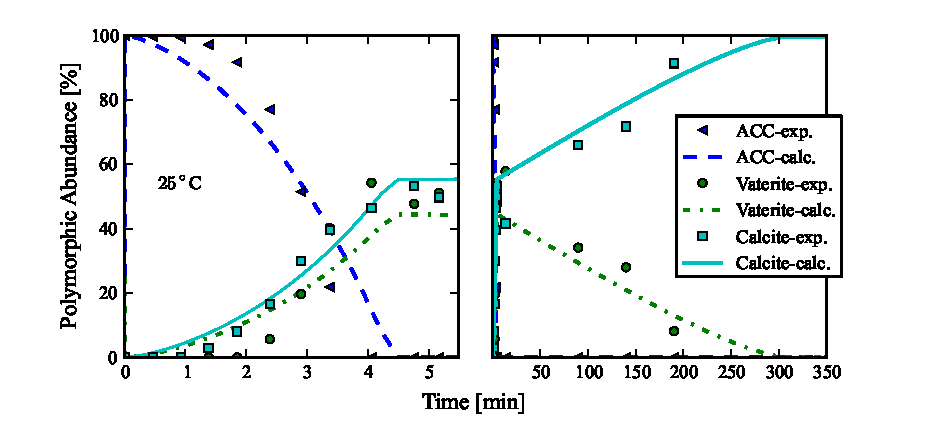
\includegraphics{fig_5_PA_optimized_tensions_25C}
\end{center}
\caption{Polymorphic abundance traces over time at $25^\circ$C, where calculated data (lines) is compared to experimental data (symbols) extracted from \citep{Ogino1987}.  Experimental ACC data are shown as the triangles, calculated ACC data are the dashed lines, experimental vaterite data are the circles, calculated vaterite data are the dash-dot lines, experimental calcite data are the squares, and calculated calcite data are the solid line.  Aragonite values are near zero throughout time in both plots.  Interfacial tension values used within the framework were optimized to fit experimental data at $25^\circ$C with greater emphasis on the short term timescale values.}
\label{optimized_25}
\end{figure}

Fig.~\ref{optimized_25} depicts polymorphic abundances at $25^\circ$C and compares calculated profiles with experimental data extracted from \citep{Ogino1987}.  The polymorphic abundance data calculated for Fig.~\ref{optimized_25} utilized interfacial tension values optimized to fit the $25^\circ$C experimental data, with greater emphasis on the short timescales.  The framework configuration for this figure consisted of aggregation, mixing, and diffusion limited kinetics for growth and dissolution of all \ce{CaCO3} forms except ACC's dissolution that used a kinetically limited rate in the form of Eq.~\ref{surface_growth} with the rate constant listed in Table~\ref{properties_table}.  This simple configuration captured slopes and timescales reasonably well to be utilized as a standard for comparison.    
%After trying diffusion limited and other kinetically limited mechanisms and rate constants, the aforementioned form was found to best capture the slopes and timescales presented in \cite{Ogino1987}.

Although the profiles shown in Fig.~\ref{optimized_25} do an adequate job of matching the experiment data, their inconsistencies can be used as points of comparison with alternative configurations.  These inconsistencies include ACC's polymorphic abundance not remaining near 100$\%$ polymorphic abundance until $\sim$1.5 minutes, vaterite crossing over calcite's polymorphic abundance at $\sim$3.5 minutes, and resultant dampened slopes.  
%Throughout the framework are many particle physics components that can be implemented, but 
The two most fundamentally significant options explored during framework development dealt with the selection of the growth and nucleation mechanisms.

\begin{figure}[!htbp]
\begin{center}
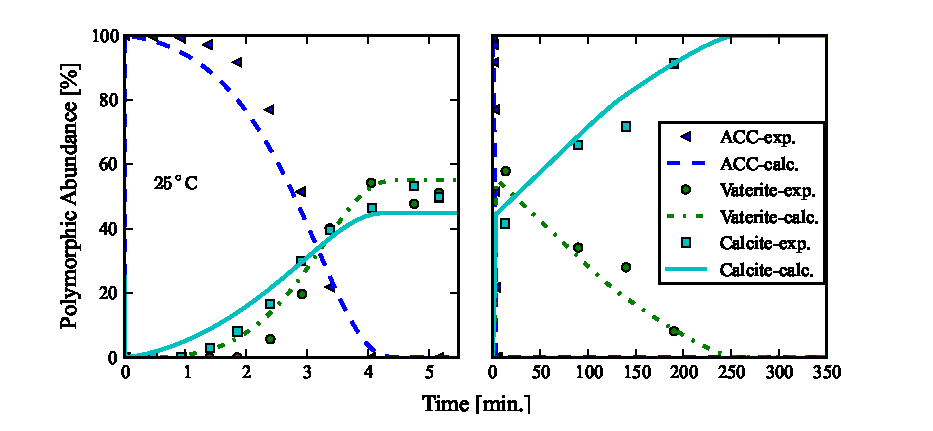
\includegraphics{fig_6_heterogeneous_nucleation}
\end{center}
\caption{Polymorphic abundances at $25^\circ$C calculated utilizing simultaneous heterogeneous and homogeneous nucleation models with fitted interfacial tensions and heterogeneous nucleation parameters.  Growth and dissolution mechanisms were diffusion based.  Calculated data (lines) is compared with experimental data extracted from \citep{Ogino1987} (symbols).  Experimental ACC data are shown as the triangles, calculated ACC data are the dashed lines, experimental vaterite data are the circles, calculated vaterite data are the dash-dot lines, experimental experimental calcite data are the squares, and calculated calcite data are the solid line.  A purely homogeneous nucleation equivalent can be seen in Fig.~\ref{optimized_25}.}
\label{hetero}
\end{figure}
Heterogeneous nucleation is believed to be present in the system of interest, but the magnitude of its contribution is not known.  Fig.~\ref{hetero} depicts how simultaneous implementation of heterogeneous and homogeneous nucleation allows the calculated system to more closely reproduce the polymorphic abundance profiles found in \citeauthor{Ogino1987} including the delays of calcite and vaterite growth, the cross over of the two polymorphs at around $3.5$ minutes and the general slopes of each polymorph's volumetric abundance.  The implementation of heterogeneous nucleation introduces unknown parameters, which along with interfacial tension values were optimized to produce Fig.~\ref{hetero}.  Although  the results give credibility to the idea that a significant amount of heterogeneous nucleation may be occurring in the system, the heterogeneous nucleation model adds too many degrees of freedom to the framework to be conclusive.  In order to avoid overfitting, only homogeneous nucleation was used in the final framework.
\begin{figure}[!htbp]
\begin{center}
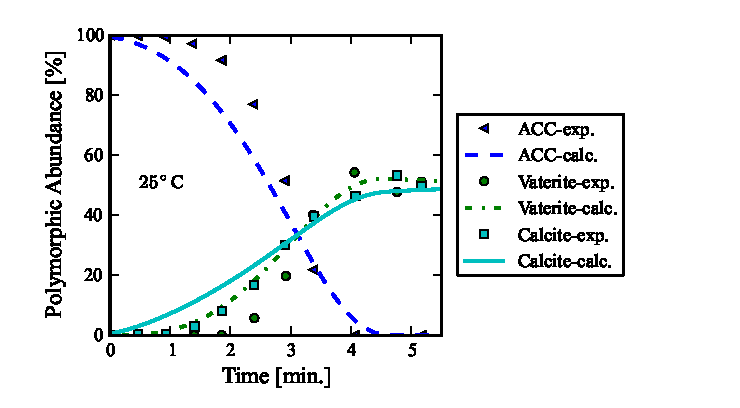
\includegraphics{fig_7_dual_growth_mechanism}
\end{center}
\caption{Polymorphic abundances at $25^\circ$C calculated, where vaterite's growth mechanism switched from diffusion limited to a screw dislocation mechanism at a supersaturation value of 47, all other growth and dissolution mechanisms were diffusion based and interfacial tensions were fitted.  Calculated data (lines) is compared with experimental data extracted from \citep{Ogino1987} (symbols).  Experimental ACC data are shown as the triangles, calculated ACC data are the dashed lines, experimental vaterite data are the circles, calculated vaterite data are the dash-dot lines, experimental calcite data are the squares, and calculated calcite data are the solid line.}
\label{alt_grow}
\end{figure}

Other possible framework configurations include implementing different growth and dissolution mechanisms or switching between mechanisms as was mentioned in Sec.~\ref{Grow_Section}.  Fig.~\ref{alt_grow} demonstrates how a transition between growth mechanisms captures dynamics that were absent from the calculated profiles in Fig.~\ref{optimized_25}.  For the simulation shown in Fig.~\ref{alt_grow}, a transition in vaterite's growth mechanism from diffusion limited to screw dislocation occurs at a supersaturation value of 47 and the interfacial tension values were again fitted.  Using multiple growth mechanisms for vaterite allows for the short term crossover behavior to be captured, but choosing a transition point is somewhat arbitrary and similar behaviors can be observed for a range of supersaturation values by altering interfacial tension values.  Other growth mechanisms not currently being considered would be transitioned through in between these two mechanisms.  The multiple growth mechanism implementation captures polymorphic abundance slopes that bear a closer resemblance to the experimental data.  Unfortunately, the simulations run using multiple growth mechanisms for vaterite and/or aragonite had long term behaviors that were extensively longer than the validation data, so this tendency would also need to be overcome for general implementation.  

Due to the extent of recent research on calcite's growth and dissolution rates, more complex mechanisms from literature sources were considered.  \cite{Wolthers2012}'s mechanism, with ionic ratio and pH dependence, was implemented for calcite's growth at low supersaturation.  A transition between diffusion limited and \citeauthor{Wolthers2012}'s kinetically limited mechanism was found to function well at a supersaturation around 1.5.  Due to the incorporation of temperature dependence into \cite{Plummer1978}'s model, it was implemented for the validation case.

%Enacting a growth mechanism shift requires greater understanding of when such a transition would occur.  Thus, the growth mechanism shift was not implemented in the basic framework, but is a likely source of error.  
%Permutations of diffusion-limited, screw-dislocation, and a generic kinetically-limited models were also examined as possible dissolution mechanisms.  Ultimately it was found that using only diffusion-limited dissolution requiring no additional uncertain variables, while also resulting in the best fit to experimental traces.  

\subsection{Optimized Results}
\label{Model_Results}

The final framework was configured with mixing, homogeneous nucleation (without time lag), aggregation, diffusion limited growth for all \ce{CaCO3} forms except calcite at supersaturations below 1.5 where \cite{Wolthers2012}'s mechanism is used, kinetically limited dissolution rate in the form of Eq.~\ref{surface_growth} with the rate constant listed in Table~\ref{properties_table} for ACC, diffusion limited dissolution for vaterite and aragonite, and \cite{Plummer1978}'s dissolution mechanism for calcite.  A Nelder-Mead optimization was utilized to fit the intercept and slope parameters of the interfacial tension model (described in Sec.~\ref{interfacial_tension}).  The error kernel being minimized is based on the root square error between the polymorphic abundance and IAP extracted experimental data at all temperatures provided within \citep{Ogino1987}.  
%Comparing the optimized interfacial-tension values (Table~\ref{optimized_table}) with the range of values found in the literature (Table~\ref{tension_table}) confirms that the optimized values are near the expected range.  
Fig.~\ref{allTemps} demonstrates the performance of the optimized parameters for the interfacial tension model over a wide range of temperatures and gives a visual of part of the error kernel utilized.  
%The performance at $40^\circ$C has the worst matching, which can likely be correlated with the interfacial tension approximation that is also shown in Fig.~\ref{metastable}.  %the profiles for all temperatures are satisfactorily captured.

\begin{table}[ht]
\caption{Interfacial tension model parameters from optimization}
\centering
\begin{tabular}{c | c | c}
\hline\hline
Polymorph & $\sigma_{25^\circ\text{C}, \mu^\circ} [\text{mJ} \; \text{m}^{-2}]$ & $-S_a^E \; [\text{mJ} \; \text{m}^{-2} \; \text{K}^{-1}]$ \\ 
\hline
ACC & -12.6 & $2.47 \times 10^{-2}$ \\
Vaterite & 64.6 & $3.57 \times 10^{-2}$ \\
Aragonite & 96.3 & $-3.16 \times 10^{-1}$ \\
Calcite & 8.94 & $1.06 \times 10^{-1}$ \\
\hline
\end{tabular}
\label{optimized_table}
\end{table}

One means of visualizing and gauging the success of the interfacial tension model with the optimized parameter values is the metastable polymorphic abundances across the experimental temperature range. The metastable stage is interpreted as occurring after the majority of ACC dissolves and the IAP plot reaches its second flat region (see Fig.~\ref{IAP}).  A table of times to reach the metastable stage was included in \citet{Ogino1987} and was used to define the framework produced polymorphic abundances in Fig.~\ref{metastable}.  The metastable stage can be seen in Fig.~\ref{IAP} as occurring around six and three minutes for the $25^\circ$C and $50^\circ$C systems.  Fig.~\ref{metastable} substantiates the performance of the interfacial tensions model by overlaying the results on the metastable polymorphic abundances observed by \citeauthor{Ogino1987}  The short time-scales of the higher temperatures have better agreement with the experimental data, but the qualitative shapes were captured -- albeit dampened in amplitude.  Deviations between the calculated values and the experimental data can be attributed to a compound effect of the approximations and assumptions introduced within the framework.  As was discussed in Sec.~\ref{Grow_Section}, there is a large body of literature on calcite's dissolution mechanism.  Unfortunately, there is far less information available on temperature and composition dependent dissolution mechanisms of the three other forms of \ce{CaCO3}.  Approximating ACC's dissolution rate with a temperature independent kinetically limited model and vaterite and aragonite's dissolution rates as diffusion limited is likely a key factor in the poor performance of the long timescales.
%One such approximation is the independence of interfacial tension from the solution composition, yet for such a major assumption this framework preforms notably well.  Exceptions are the results at $30^\circ$C and $40^\circ$C, but these do correlate with the poor agreement seen in the polymorphic abundances for $40^\circ$C. 

\begin{figure}[!htbp]
\begin{center}
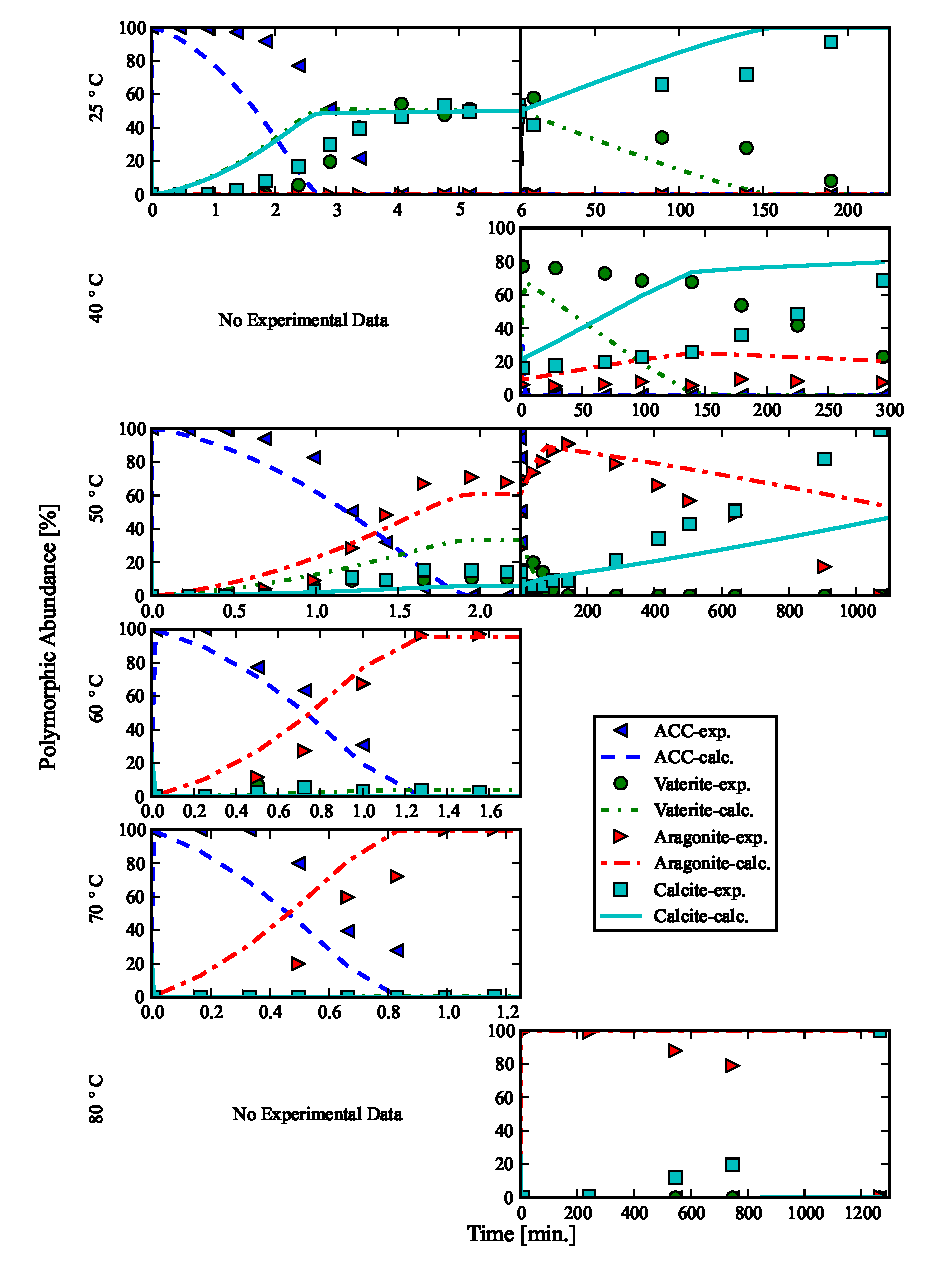
\includegraphics[scale=.85]{fig_8_PA_all_temperatures}
\end{center}
\caption{Comparison of calculated polymorphic abundance traces (lines) over time with all polymorphic abundance data presented within \citep{Ogino1987} (symbols), which range over temperatures.  Experimental ACC data are shown as the left pointing triangle, calculated ACC data are the dashed lines, experimental vaterite data are the circles, calculated vaterite data are the shorter dash-dot lines, experimental aragonite data are the right facing triangles, calculated aragonite data are the longer dash-dot lines, experimental calcite data are the squares, and calculated calcite data are the solid line.  The calculated profiles shown reflect points utilized in optimization search of interfacial tension model parameter space.}  
\label{allTemps}
\end{figure}

\begin{figure}[!htb]
\begin{center}
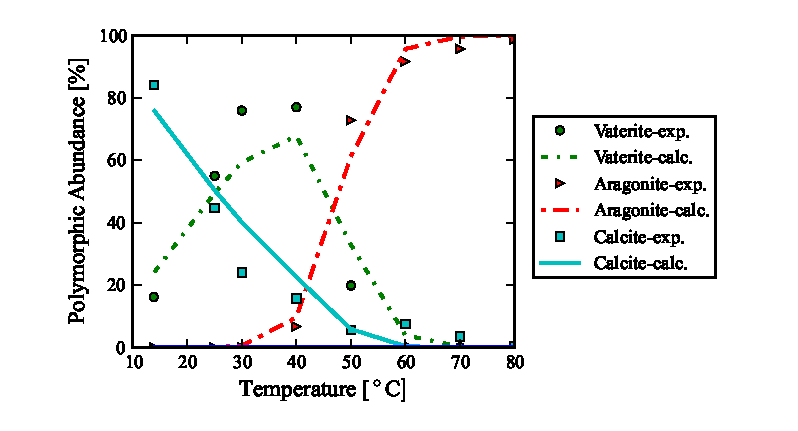
\includegraphics{fig_9_PA_metastable}
\end{center}
\caption{ Comparison of calculated polymorphic abundance traces (lines) at the metastable stage with experimental data from \citep{Ogino1987} (symbols) over a range of temperatures.  The time at which the system reaches the metastable stage is defined as once the system's IAP levels out after the majority of ACC has dissolved.  Experimental vaterite data are the circles, calculated vaterite data are the shorter dash-dot lines, experimental aragonite data are the right facing triangles, calculated aragonite data are the longer dash-dot lines, experimental calcite data are the squares, and calculated calcite data are the solid line.  The tabulated times from \citep{Ogino1987} were used to determine the calculated data except for $13^\circ$C, which has to use a longer time due to ACC still being significantly present in the system at the tabulated time.}
\label{metastable}
\end{figure}

The IAP plots shown in Fig.~\ref{IAP} can be used to observe the general timescales at which processes are occurring.  Within Fig.~\ref{IAP} calculated IAP traces are compared with experimental data extracted from \cite{Ogino1987} and that data once correlated with \cite{Cantera}'s chemistry.  The experimental data has poor agreement with initial calculated IAP.  It can be noted that during the initial drop in IAP, nucleation of all forms of \ce{CaCO3} is occuring, but the experimental data remains above ACC's solubility prior to ACC's dissolution.  Once correlated the IAP trace settles to values below ACC's solubility.  When multiple polymorphic forms are present, the IAP values are expected to be below the solubility line of the currently least stable polymorph, which initially is ACC.  The IAP then maintains a generally flat trend until the majority of ACC has dissolved.  Such flat trends are known as meta-stable periods. Then the IAP drops near to the next least stable polymorph's solubility, which is vaterite for both cases shown.  This process is repeated for aragonite and calcite with differing lengths of metastability between drops, except at $25^\circ$C where aragonite's metastable region is not present due to aragonite's instability at this temperature.  Although the correlated data performs well near ACC and vaterite's solubilities, the correlated IAPs become overly low when aragonite and calcite are predominate.  There are many possible explanations for this occurrence, one being probe fouling.

%During the initial drop in IAP, nucleation of all forms of \ce{CaCO3} is occurring and the IAP settles near a value representative of ACC's solubility, due to ACC's predominance in the system at that time.  When multiple polymorphic forms are present, the IAP values are below the solubility line of the currently least stable polymorph.  

%Fig.~\ref{IAP} compares the calculated IAP results with \citeauthor{Ogino1987}'s experimental results. 
The general behaviors of the IAP and polymorphic abundance curves were all captured reasonably well considering the basic models used for the particle physics and the assumptions made throughout the framework.  It is noteworthy that primarily using diffusion limited growth and dissolution models was able to capture the general short timescales of the process at a variety of temperatures as can be seen in Fig.~\ref{allTemps}.  Although many other kinetic mechanism are known to be present in \ce{CaCO3} systems, the high initial supersaturation allowed the short time scales to be captured well with diffusion based models.  Calcite had additional kinetic models enacted for its dissolution and growth, but due to the system approaching equilibrium, they had minor effects.  

%This is of interest because at $50^\circ$C there is a quicker short-term transition to the metastable state than at $25^\circ$C and there is an extended long timescale to reach the stable state than at $25^\circ$C.

\begin{figure}[h!tb]
\begin{center}
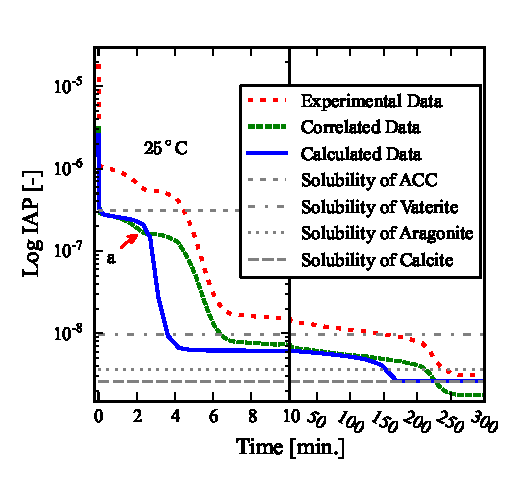
\includegraphics{fig_10a_IAP_25C}
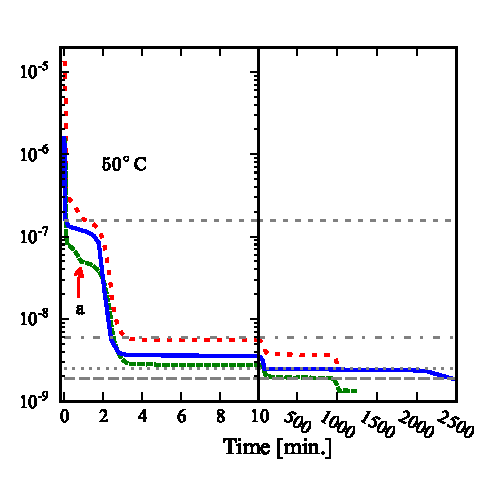
\includegraphics{fig_10b_IAP_50C}
\end{center}
\caption{Ion activity product traces at $25^\circ$C and $50^\circ$C over time, comparing experimental and correlated data from \citep{Ogino1987} (wide gaped and narrow gaped dotted lines respectively) and calculated profiles (solid line).  The solubilities of each polymorph are also shown for comparison with meta-stable periods (flat trends) of the particle population, where the shorter dashed lined is ACC's solubility, the dash-dot line is vaterite's solubility, the doted line is aragonite's solubility, and the longer dashed line is calcite's solubility.  Arrows point to `a' inflection points that are caused by an unknown particle phenomena and are not captured by framework.} 
\label{IAP}
\end{figure}

In the IAP plots provided by \citeauthor{Ogino1987}, the information for the initial seconds of the reaction is masked and unclear due to the reported data's time resolution.  There is a large drop in the IAP, but this is shown to occur in less than one minute.  Resolved data for the initial seconds of the experiment could allow for greater understanding of mixing and nucleation within the system.  In both IAP plots of the original data there are noticeable and unexplained inflection points, prior to reaching the metastable stage, labeled in Fig.~\ref{IAP} with an `a'.  The current approach is unable to recreate the `a' inflection points, but it seems plausible that a secondary form of ACC could be the cause as discussed in \citep{Cartwright2012,Radha2010} .  Alternative causes of the inflection points include a change in the dissolution mechanism of ACC, a bimodal ACC distribution, non-classical nucleation, or a connection with heterogeneous nucleation.  

To further support the possibility of an additional variety of ACC existing, it can be noted that prior to the `a' inflection point, the IAP curve correlated from \citeauthor{Ogino1987} is slightly below the known solubility of ACC at $25^\circ$C and $50^\circ$C, while after the 'a' inflection point the IAP stabilizes at a value still well above vaterite's solubility.  All of the other inflection points on the IAP curves correspond to reaching metastable states, so it is reasonable to assume that the observed inflection point also corresponds to a new metastable state.   The final dip in the IAP curves, corresponding to the final transformation to pure calcite, is notably late for the calculated data.  This discrepancy can be better understood through analysis of the polymorphic abundance plots.

The polymorphic abundance plots (Fig.~\ref{allTemps}) reveal another physical phenomena during the initial $1.0-2.0$ minutes at $25^\circ$C, $0.5-0.75$ minutes at $50^\circ$C and until near 0.3 minutes at $60^\circ$C and $70^\circ$C, which the current particle physics models do not capture.  This phenomena can be viewed as a longer period of stability for ACC or as a delay in the nucleation and growth of the other polymorphs.  A longer period of ACC stability could also be expected if two forms of ACC were lumped together when calculating polymorphic abundances.  Nucleation induction times were investigated as the cause of the delay, but the order of magnitude required to have a similar effect clashes with timescales predicted in the literature \citep{Kashchiev1969}.  Other possible explanations include an under-prediction of the initial ACC nucleation or the nucleation of the polymorphs being heterogeneous rather than homogeneous.  While the cause of the delay remains undetermined, it is evidently a temperature dependent phenomena that becomes less influential with increased temperatures.  As a repercussion of not capturing the initial delay with the particle physic models, the interfacial tension values found to best capture the overall system timescales cause the short and long timescale polymorphic abundances to have deviation from the experimentally found values and the slopes generated by the framework were generally dampened.  
%When modeling the system without the initial delay, smaller interfacial tension values can be found that allow for better matches to the long and short timescale data and slopes that have an improved resemblance to the experimental results.

For temperatures $25^\circ$C and $50^\circ$C as depicted in Fig.~\ref{allTemps}, there is a point at which (as observed in the experimental but not calculated data) the polymorphic abundance of vaterite becomes more prevalent than that of calcite.  This crossover occurs on the short term timescale and then reverses in the long term.  The short term crossover at $50^\circ$C is not shown on the plot itself, but can be deduced from the polymorphic abundances on the long term plot and metastable polymorphic abundances shown in Fig.~\ref{metastable}.  While the crossovers in the long term plots are due to calcite being the most stable polymorphic form, the short term crossover could be attributed heterogeneous nucleation or to a shift in growth mechanism as was demonstrated in Sec.~\ref{Model_Alternatives}.

\section{Conclusions}
An overarching mathematical framework has been proposed to describe complex precipitation processes.  The described system involved the evolution of multiple polymorphic forms over a range of temperatures.  Within the framework, models describing individual physical phenomena effecting the precipitation process such as nucleation and growth, are coupled with an aqueous ionic equilibrium-chemistry model and a mixing model, in order to capture complete multiphase system dynamics.  The framework presented can provide multiple outputs, not all of which had corresponding validation data, that are of interest within precipitation studies such as PSDs.   Additional framework configurations could be tested with alternative physical or chemical models such as a non-classical nucleation models.  

Ultimately, a simple configuration that minimizes error over unknown variables was implemented to display the framework's strength.  Through calculated results inter-polymorph effects were observed as well as dynamics within each polymorph's own PSD such as Oswald ripening.  When utilizing optimized parameters for the interfacial tension model, the framework was validated through comparison with \citet{Ogino1987}'s experimental data.  The framework, while only fitting interfacial tension parameters, produced results that resembled the temperature varying experimental data even with known assumptions and uncertainties.  This framework could be used by experimentalists to further explore currently relevant physical phenomena such as heterogeneous nucleation and non-classical nucleation.

\section*{Acknowledgments}
We would like to acknowledge the help and insights of Dr. T. Ring and Dr. T. Saad.

\bibliography{CaCO3Collection.bib}

\end{document}
